\documentclass[11pt,reqno]{amsart}

\usepackage[margin=0.9in]{geometry}
\usepackage{amsmath,amssymb}
\usepackage{booktabs}
\usepackage{array}
\usepackage{tabularx}
\usepackage{enumitem}
\usepackage{xcolor}
\usepackage{graphicx}
\usepackage{microtype}
\usepackage{tikz}
\usepackage{pgfplots}
\pgfplotsset{compat=1.18}
\usetikzlibrary{arrows.meta,positioning}
\usepackage[hidelinks]{hyperref}

\emergencystretch=2.5em

\definecolor{azblue}{RGB}{24,78,119}
\definecolor{azteal}{RGB}{22,138,173}
\definecolor{azslate}{RGB}{65,78,94}
\definecolor{azamber}{RGB}{186,112,24}
\definecolor{azlight}{RGB}{242,246,250}

\newcommand{\tagbadge}[1]{\textsc{\scriptsize #1}}
\newcommand{\code}[1]{\texttt{\footnotesize #1}}
\newcommand{\us}{\_\allowbreak}
\newcommand{\slsh}{/\allowbreak}
\newcolumntype{L}[1]{>{\raggedright\arraybackslash}p{#1}}
\newcolumntype{Y}{>{\raggedright\arraybackslash}X}

\title[Asmodensius-Native v1.1.0]{Asmodensius-Native: A Freestanding C23, AVX-VNNI, and Pure-Integer PTX Artificial-Life Engine with 6-Kernel Lean 4.35.0 Formal Invariants}

\author{Alexander Stephen Donahue}
\address{Independent Researcher, Spokane, WA, USA}
\email{0\_0@0thernes.art}
\urladdr{https://orcid.org/0009-0006-8168-9648}

\date{November 25, 2026 (Version 1.1.0 Preprint -- Not Peer-Reviewed)}

\subjclass[2020]{Primary 68T42, 68N30; Secondary 68Q60, 92D15, 68W10}
\keywords{Artificial life, freestanding C23, integer conservation, Philox4x32-10, AVX-VNNI, CUDA PTX, deterministic simulation, Lean 4 formal verification}

\begin{document}

\begin{abstract}
We present \code{Asmodensius-Native} v1.1.0, a Windows-native, freestanding C23 artificial-life simulation engine designed for cache-resident, single-arena, integer-only execution at populations from $1$ to $1{,}004{,}019$ live digital organisms without virtual machines, language models, pretrained weights, floating-point simulation arithmetic, or pagefile backing. The engine comprises $22$ selectable freestanding core biology and physics modules plus $4$ pure-integer mathematical kernels (\code{tk\us*}), $4$ NASM x86-64 AVX2/AVX-VNNI assembly twins, and a Clang~21 \code{nvptx64} pure-integer CUDA PTX device module ($41{,}817$~bytes, $0$~external calls, $0$~floating-point instructions) compiled directly from the same freestanding C23 sources. Worlds execute in \emph{wild} mode by default (drawing fresh OS entropy every tick) and in \emph{lab} mode (\code{--lab}) using counter-based Philox4x32-10 streams for bit-exact state-hash parity across thread counts, reorder schedules, CPU SIMD twins, and RTX~5070~Ti GPU offload.

Verification spans two explicitly separated layers: (i)~\emph{empirical software and hardware verification}, comprising $77/77$ passing CTest targets (including UBSan trap builds, stack-usage and object-symbol gates, and multi-substrate determinism matrices) and $164/164$ passing GPU differential checks over $1{,}000{,}000$ variable-size sparse brains and $1{,}000{,}000$ kinematics lanes ($0$~differing bits); and (ii)~\emph{machine-checked formal verification} of $30$ core conservation, refusal, ABI, Philox-key, and VRAM-addressing theorems (\code{A01}--\code{A30}) in pure Lean~4.35.0 (zero Mathlib, zero \code{sorry} in \code{Solution}, zero \code{native\us decide}) architected for isolated \code{Challenge}\slsh\code{Solution} 6-kernel Palomar auditing. Measured bare-metal throughput on an Intel Core Ultra~9~275HX ($8\text{P}+16\text{E}$) and NVIDIA RTX~5070~Ti demonstrates $+56.7\%$ speedup at $100\text{k}$ founders ($72.199$~ms/tick on 24C AVX-VNNI+PF) and $+35.3\%$ at $1\text{M}$ founders ($757.988$~ms/tick, $9{,}260.6$~MB page-locked), while honestly disclosing PCIe and compaction overhead where 24C CPU beats GPU at $1\text{M}$ ($1{,}122.495$~ms/tick) and Windows \code{SeLockMemoryPrivilege} fallback for 2~MB large pages. This paper is an unrefereed independent technical preprint: it makes zero claims of sentience, consciousness, biological life, or quantum speedup, and retires $0/1{,}900$ overarching problems in the Unsolved Problems Mega-Atlas.
\end{abstract}

\maketitle

\section{Introduction and Epistemic Scope}

Artificial-life (ALife) platforms such as Tierra~\cite{ray1991approach}, Avida~\cite{ofria2004avida}, and indefinitely scalable spatial engines~\cite{ackley2014indefinitely} established that computational ecosystems can probe evolutionary dynamics, resource competition, and open-endedness~\cite{bedau2000open,taylor2016open,packard2019overview}. Yet modern ALife simulators frequently trade away strict numerical conservation, cross-hardware determinism, or low-level memory predictability in favor of managed runtimes, floating-point drift, or opaque neural controllers.

\code{Asmodensius-Native} explores an opposite engineering regime governed by $15$ explicit project laws (\code{AGENTS.md}):
\begin{enumerate}[leftmargin=2.0em,itemsep=2pt]
  \item \textbf{Freestanding native simulation:} the core (\code{core/}) compiles under ISO C23~\cite{iso2024c23} with \code{-ffreestanding}, zero libc calls, zero heap allocation, zero floating-point operations, and enforced stack frames $\le 2{,}048$~bytes.
  \item \textbf{Single page-locked arena:} all simulation state resides in one pre-allocated, Windows \code{VirtualLock}-pinned arena structured as cache-aligned Structure-of-Arrays (SoA) blocks (\code{AZ\us CHUNK = 128}) without pagefile or NVMe swap backing.
  \item \textbf{Exact integer conservation:} matter and energy are tracked as exact integers; both global balance equations must hold with \code{==} after every tick, with \code{field\us underflow == 0} and \code{dropped\us events == 0}.
  \item \textbf{Wild default with bit-exact lab replay:} unflagged runs draw fresh OS entropy every tick; \code{--lab} runs use Philox4x32-10~\cite{salmon2011parallel} keyed by seed and canonical \code{uid} ordering so scalar C, AVX2/AVX-VNNI twins, and CUDA PTX kernels produce identical 64-bit \code{az\us state\us hash} outputs.
  \item \textbf{No borrowed intelligence and strict indicator-only reporting:} zero LLMs, pretrained weights, or designer fitness functions enter the engine; every mechanism must carry an explicit lesion bit, and cognitive diagnostics follow an indicator-only discipline~\cite{butlin2023consciousness} with zero claims of sentience or life.
\end{enumerate}

Table~\ref{tab:claims} summarizes the numbered claims ledger (\code{CLAIMS.md}), attaching explicit epistemic tiers and concrete falsification conditions to every statement in this paper.

\begin{table}[htbp]
\centering
\caption{Numbered Claims Ledger with Epistemic Tiers and Refutation Criteria.}
\label{tab:claims}
\footnotesize
\setlength{\tabcolsep}{4pt}
\begin{tabularx}{\textwidth}{L{0.65cm}L{2.25cm}YY}
\toprule
\textbf{ID} & \textbf{Tier} & \textbf{Scoped Claim} & \textbf{What Would Refute It} \\
\midrule
C01 & \tagbadge{kernel-checked} & 30 Lean~4.35.0 theorems (\code{A01}--\code{A30}) compile with 0 \code{sorry} in \code{Solution}, 0 \code{native\us decide}, and axioms $\subseteq \{\text{propext}, \text{Classical.choice}, \text{Quot.sound}\}$. & Any forbidden axiom, kernel rejection by \code{leanchecker-paranoid}, \code{con-leche}, \code{con-ron}, \code{nanoda\us bin}, or \code{lean4lean}. \\
C02 & \tagbadge{kernel-checked} & Guard boundaries \code{acceptSpecies} ($1\dots 100$) and \code{uid < 2\^{}32} for bulk Philox key equivalence are strictly necessary (\code{A29}, \code{A30}). & A proof that unrestricted \code{req} or \code{uid >= 2\^{}32} preserves acceptance or key identity. \\
C03 & \tagbadge{program-audited} & Freestanding \code{az\us core} links zero FP ops, zero writable globals, stack frames $\le 2048$~B, and passes $77/77$ CTest targets including UBSan traps. & Any failure in \code{core\us obj\us gate}, \code{avx\us stack\us gate}, \code{lint\us core}, \code{ubsan\us trap\us build}, or any CTest target. \\
C04 & \tagbadge{program-audited} & Clang~21 \code{nvptx64} PTX ($41{,}817$~B) has 0 externs and 0 floats; \code{test\us gpu} passes $164/164$ with 0 differing bits across $10^6$ brains and $10^6$ kinematics lanes. & Any non-zero diff in \code{test\us gpu.exe} or any \code{.extern}/\code{.f32}/\code{.f64} instruction in \code{az\us gpu\us dev.ptx}. \\
C05 & \tagbadge{empirical} & Bit-exact \code{az\us state\us hash} parity holds across C-ref, AVX-VNNI+Philox, 24C P+E, and RTX~5070~Ti GPU at $1\text{k}$, $10\text{k}$, $100\text{k}$, and $1\text{M}$ founders. & Any single-bit hash divergence between \code{--kernels 0}, \code{--kernels 1}, \code{--ecores}, or \code{--gpu 1} on identical \code{--lab} seeds. \\
C06 & \tagbadge{empirical} & On Core Ultra~9~275HX, 24C AVX-VNNI+PF reaches $72.199$~ms/tick at $100\text{k}$ ($+56.7\%$) and $757.988$~ms/tick at $1\text{M}$ ($+35.3\%$, $9{,}260.6$~MB locked). & Interleaved clean-machine repeats showing regression or unlocked arena (\code{locked=0}) at matched config. \\
C07 & \tagbadge{empirical} & GPU offload at $1\text{M}$ founders is slower ($1{,}122.495$~ms/tick) than 24C CPU ($757.988$~ms/tick) due to PCIe/compaction overhead (negative tradeoff). & A valid locked-arena GPU run at $1\text{M}$ without store-layout change outperforming 24C CPU. \\
C08 & \tagbadge{indicator-only} & Evaluation catalogs (\code{butlin14}, \code{cqm25}, \code{MECHANISMS.csv}) measure mechanistic indicators only; reserved blocks $5001$--$5024$ and $6001$--$6124$ remain unburned. & Any claim of sentience/AGI or unlogged confirmation execution on reserved seeds. \\
C09 & \tagbadge{open-conj.} & Long-horizon open-ended evolutionary dynamics (\code{AI-045}, \code{BIO-008}) remain open; $0/1{,}900$ Mega-Atlas problems are solved or retired. & Only an independently verified mathematical proof or decisive biological/ALife consensus resolution. \\
\bottomrule
\end{tabularx}
\end{table}

\section{System Architecture and Mathematical Formulation}

\subsection{Repository and ABI v4 Layout}

The simulation core (\code{core\slsh az\us abi.h}, ABI version $4$) separates $22$ selectable domain modules (\code{rng}, \code{fx}, \code{grid}, \code{scan}, \code{sense}, \code{brain}, \code{genome}, \code{social}, \code{mate}, \code{econ}, \code{metab}, \code{physics}, \code{life}, \code{field}, \code{chem}, \code{weather}, \code{colony}, \code{tier1}, \code{stats}, \code{worldgen}, \code{ledger}, \code{snapshot}) from $5$ core runtime files (\code{az\us world.c}, \code{az\us tick.c}, \code{az\us store.c}, \code{az\us kin\us axis.c}, \code{az\us rock\us place.c}) and $4$ pure-integer mathematical kernels derived from open-source mathematical specifications: fixed-point real solid harmonics (\code{tk\us sh.c}), $64$-spin Hopfield associative memory~\cite{hopfield1982neural} (\code{tk\us hop.c}), fixed-point quantum geometric tensor (\code{tk\us qgt.c}), and a strictly classical small-state-vector simulator (\code{tk\us qsv.c}, conferring zero quantum speedup or quantum randomness).

Each organism carries a variable-length diploid genome (initial founders fitted to ecological niches~\cite{hutchinson1957concluding} on integer value-noise terrain~\cite{perlin1985image}) developing into $\code{AZ\us TRAITS} = 112$ quantitative traits and $16$ hot phenotype scalars, an articulated multi-part body stored in $64$-byte (\code{AZ\us UNIT}) cache-line granules inside a two-half compacting creature store, and a sparse tiled \code{int8} recurrent neural network mapping $\code{AZ\us SENS} = 64$ unsigned sensory inputs ($0\dots 127$) through $8$-wide hidden blocks to $\code{AZ\us MOT} = 24$ signed motor channels ($-127\dots 127$). Figure~\ref{fig:architecture} illustrates how all three compute backends execute the identical mathematical specification against one locked arena.

\begin{figure}[htbp]
\centering
\resizebox{\textwidth}{!}{%
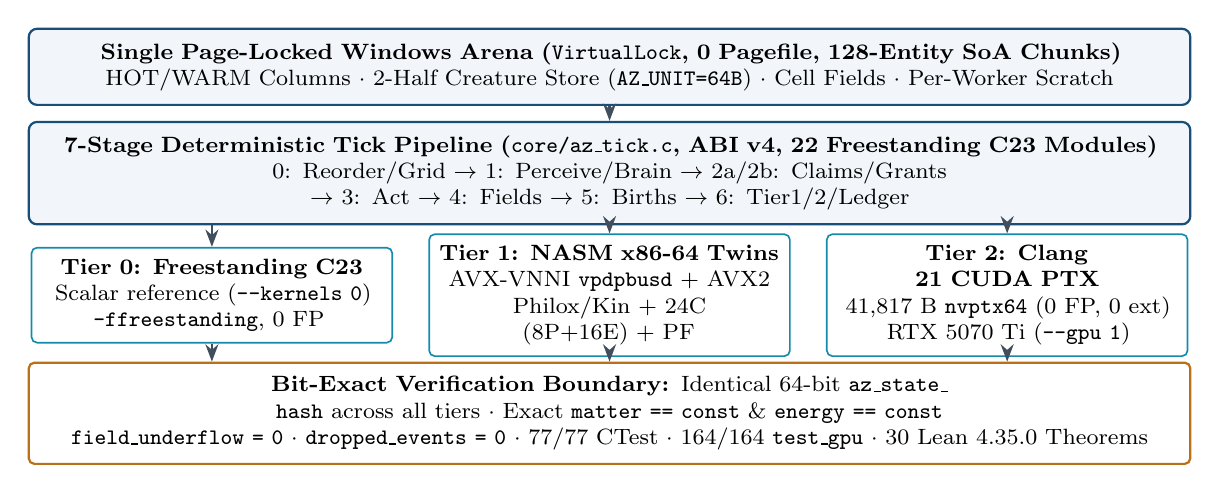
\begin{tikzpicture}[
  font=\footnotesize,
  box/.style={draw=azblue, fill=azlight, rounded corners=3pt, thick, align=center, text width=14.4cm, minimum height=0.88cm, inner sep=5pt},
  sub/.style={draw=azteal, fill=white, rounded corners=2pt, semithick, align=center, text width=4.3cm, minimum height=0.82cm, inner sep=4pt},
  gate/.style={draw=azamber, fill=white, rounded corners=2pt, thick, align=center, text width=14.4cm, minimum height=0.82cm, inner sep=5pt},
  arr/.style={-{Stealth[length=2.2mm]}, thick, color=azslate}
]
  \node[box] (arena) at (0,3.25)
    {\textbf{Single Page-Locked Windows Arena (\code{VirtualLock}, 0 Pagefile, 128-Entity SoA Chunks)}\\
     HOT/WARM Columns $\cdot$ 2-Half Creature Store (\code{AZ\us UNIT=64B}) $\cdot$ Cell Fields $\cdot$ Per-Worker Scratch};

  \node[box] (pipe) at (0,1.90)
    {\textbf{7-Stage Deterministic Tick Pipeline (\code{core/az\us tick.c}, ABI v4, 22 Freestanding C23 Modules)}\\
     0: Reorder/Grid $\to$ 1: Perceive/Brain $\to$ 2a/2b: Claims/Grants $\to$ 3: Act $\to$ 4: Fields $\to$ 5: Births $\to$ 6: Tier1/2/Ledger};

  \node[sub] (cpu0) at (-5.05,0.35)
    {\textbf{Tier 0: Freestanding C23}\\
     Scalar reference (\code{--kernels 0})\\
     \code{-ffreestanding}, 0 FP};
  \node[sub] (cpu1) at (0,0.35)
    {\textbf{Tier 1: NASM x86-64 Twins}\\
     AVX-VNNI \code{vpdpbusd} + AVX2\\
     Philox/Kin + 24C (8P+16E) + PF};
  \node[sub] (gpu1) at (5.05,0.35)
    {\textbf{Tier 2: Clang 21 CUDA PTX}\\
     41,817 B \code{nvptx64} (0 FP, 0 ext)\\
     RTX 5070 Ti (\code{--gpu 1})};

  \node[gate] (hash) at (0,-1.15)
    {\textbf{Bit-Exact Verification Boundary:} Identical 64-bit \code{az\us state\us hash} across all tiers $\cdot$ Exact \code{matter == const} \& \code{energy == const}\\
     \code{field\us underflow = 0} $\cdot$ \code{dropped\us events = 0} $\cdot$ 77/77 CTest $\cdot$ 164/164 \code{test\us gpu} $\cdot$ 30 Lean 4.35.0 Theorems};

  \draw[arr] (arena.south) -- (pipe.north);
  \draw[arr] (pipe.south -| cpu0.north) -- (cpu0.north);
  \draw[arr] (pipe.south) -- (cpu1.north);
  \draw[arr] (pipe.south -| gpu1.north) -- (gpu1.north);
  \draw[arr] (cpu0.south) -- (hash.north -| cpu0.south);
  \draw[arr] (cpu1.south) -- (hash.north);
  \draw[arr] (gpu1.south) -- (hash.north -| gpu1.south);
\end{tikzpicture}%
}
\caption{Asmodensius-Native v1.1.0 single-arena multi-substrate architecture. Every compute backend compiles from or checks against the freestanding C23 core and converges on bit-exact \code{az\us state\us hash} parity.}
\label{fig:architecture}
\end{figure}

\subsection{Exact Integer Conservation Laws}

Let $M_{\mathrm{bio}}(t)$ denote total organic biomass across all living entity pools, $M_{\mathrm{cell}}(t)$ total field, inventory, colony-store, and reservoir matter, $E_{\mathrm{bio}}(t)$ total entity internal energy, and $H_{\mathrm{cell}}(t)$ total cell thermal heat. Each matter species carries a fixed integer chemical potential $\varepsilon_s \in \mathbb{N}$ defined in \code{core\slsh az\us abi.h}:
\begin{equation}
  \varepsilon(\text{NUT\_X}) = 24, \quad
  \varepsilon(\text{ORG\_Y}) = \varepsilon(\text{BIO}) = 16, \quad
  \varepsilon(\text{TOX\_Z}) = 4, \quad
  \varepsilon(\text{WST\_W}) = 2,
\end{equation}
with $\varepsilon = 0$ for solvent, gas, oxidizer, structural rock, and buried reservoir. After every tick $t \ge 0$, the runtime enforces exact equality (not tolerance bounds):
\begin{align}
  M_{\mathrm{tot}}(t) &= M_{\mathrm{bio}}(t) + M_{\mathrm{cell}}(t) = M_{\mathrm{tot}}(0), \\
  E_{\mathrm{tot}}(t) &= E_{\mathrm{chem}}(t) + E_{\mathrm{bio}}(t) + H_{\mathrm{cell}}(t) - E_{\mathrm{in}}(0..t) + E_{\mathrm{out}}(0..t) = E_{\mathrm{tot}}(0),
\end{align}
where $E_{\mathrm{in}}$ and $E_{\mathrm{out}}$ accumulate light/geothermal intake and radiative cooling in per-worker tallies merged serially at tick end. Three local accounting rules enforce global conservation and zero underflow:
\begin{itemize}[leftmargin=1.8em,itemsep=2pt]
  \item \textbf{Rule C2 (Chemical-Thermal Closure):} transforming $k$ units of \code{NUT\us X} ($24$~eu/mu) into biomass ($16$~eu/mu) simultaneously credits $(24 - 16)k = 8k$~eu into entity energy or cell heat.
  \item \textbf{Rule C5 (Receive Cap Overflow Conservation):} when a receiver at pool level $c \le C$ receives $q$ units, it retains $r = \min(q, C - c)$ and posts $q - r$ to its local cell in the same statement block, ensuring $r + (q - r) = q$ and $c + r \le C$.
  \item \textbf{Rule C7 (Six-Face Diffusion Bound):} each of the $6$ face outflows from a cell holding $A$ units is bounded by $\lfloor A / 8 \rfloor$, guaranteeing $\sum_{i=0}^{5} f_i \le 6 \lfloor A / 8 \rfloor \le A$ so \code{field\us underflow} cannot occur.
\end{itemize}

\subsection{Wild Entropy vs. Deterministic Philox4x32-10 and CUDA PTX Twins}

In default \emph{wild} mode, the Windows host obtains cryptographic entropy via \code{BCryptGenRandom} at genesis and every tick. In \code{--lab} mode, every stochastic draw uses counter-based Philox4x32-10~\cite{salmon2011parallel} indexed by $(\text{uid}, \text{tick}, \text{stream}, \text{idx})$. Under \code{--kernels 1} (TR-13), hot loops invoke an AVX2 NASM twin (\code{kernels\slsh az\us philox\us avx2.asm}) whose 32-bit key folding computes $\text{tkey}_0 \oplus \lfloor \text{uid} / 2^{32} \rfloor$; for all $\text{uid} < 2^{32}$ this equals $\text{tkey}_0$ identically, with an explicit scalar fallback guard whenever $\text{uid} \ge 2^{32}$.

The AVX-VNNI brain twin (\code{kernels\slsh az\us brain\us vnni.asm}) emits raw \code{vpdpbusd} machine bytes~\cite{intel2024sdm} to execute exact unsigned-\code{u8} $\times$ signed-\code{i8} dot products into \code{i32} accumulators without saturation. On the GPU path (TR-18/TR-04), \code{gpu\slsh az\us gpu\us dev.c} includes \code{core\slsh az\us rng.c}, \code{core\slsh az\us brain.c}, and \code{core\slsh az\us kin\us axis.c} verbatim under Clang~21 with target \code{nvptx64-nvidia-cuda}, architecture \code{sm\us 80}, and \code{-ffreestanding}~\cite{nvidia2024ptx}, producing a self-contained $41{,}817$-byte PTX binary verified at build time to contain zero \code{.extern} declarations and zero floating-point instructions, JIT-compiled by the NVIDIA driver (API 13040) for RTX~5070~Ti (compute capability 12.0).

\section{Formal Verification and Statement-Fidelity Audit}

To machine-check core algebraic and protocol invariants independently of the C compiler and runtime tests, \code{lean/} provides a standalone Pure Lean~4.35.0~\cite{moura2021lean4} formalization with zero Mathlib dependencies, \code{autoImplicit = false}, \code{relaxedAutoImplicit = false}, \code{linter.unusedVariables = true}, and Palomar \code{module} headers:
\begin{itemize}[leftmargin=1.8em,itemsep=2pt]
  \item \code{lean\slsh AsmodensiusProofs\slsh Spec.lean}: pure ABI v4 constants and state transition definitions (zero proofs, zero \code{sorry}).
  \item \code{lean\slsh AsmodensiusProofs\slsh Core.lean}: $26$ theorems (\code{A01}--\code{A26}) proving integer conservation, C2/C5/C7 bounds, species refusal, arena rollback, store release, D7 observer invariance, TR-13 Philox key equivalence, TR-18/TR-04 GPU/CPU hash parity, TR-01 prefetch transparency, 23-bit lesion mask exactness, brain SIMD alignment, and 32~GiB VRAM offset injectivity.
  \item \code{lean\slsh AsmodensiusProofs\slsh NonVacuity.lean}: $4$ theorems (\code{A27}--\code{A30}) exhibiting concrete inhabited witnesses proving hypothesis bundles are non-vacuous, plus two adversarial refutations proving that dropping the \code{acceptSpecies} ($1 \dots 100$) bound or the \code{uid < 2\^{}32} Philox guard breaks soundness.
  \item \code{lean\slsh Challenge.lean} and \code{lean\slsh Solution.lean}: isolated statement-only specification (importing only \code{Spec.lean}) paired with the sorry-free solution via \code{lean\slsh comparator.json}.
\end{itemize}

All $30$ theorems pass \code{VerifyAxioms.lean} strictly within $\{\code{propext}, \code{Classical.choice}, \code{Quot.sound}\}$ with $0$ \code{sorryAx}, $0$ \code{Lean.ofReduceBool}, and $0$ \code{Lean.trustCompiler}. Local Windows replay verifies all $5$ Windows-capable independent checkers (\code{lean}~4.35.0, \code{leanchecker --fresh}, \code{leanchecker-paranoid --fresh}, \code{con-leche --verified}, \code{con-ron --verified}, and Rust \code{nanoda\us bin} with hard-error axiom enforcement enabled), saved verbatim in \code{results\slsh lean4-multi-kernel.txt}. Linux CI additionally runs \code{lean4lean}~\cite{carneiro2024lean4lean}, \code{lake check --paranoid}, and \code{lake comparator --config comparator.json --paranoid} inside \code{bubblewrap}.

Table~\ref{tab:fidelity} maps Lean declarations to C/PTX sources and explicitly states formalization boundaries. In particular, \code{A06}, \code{A13}, \code{A15}, \code{A16}, and \code{A20} are retained for backward compatibility as constant/arithmetic sanity checks rather than deep theorems, and C23/NASM/PTX codegen fidelity is verified empirically rather than via a verified compiler.

\begin{table}[htbp]
\centering
\caption{Statement-Fidelity Matrix Mapping Source Invariants to Lean 4.35.0 Declarations.}
\label{tab:fidelity}
\footnotesize
\setlength{\tabcolsep}{3.5pt}
\begin{tabularx}{\textwidth}{L{1.85cm}L{3.15cm}L{4.05cm}Y}
\toprule
\textbf{Theorems} & \textbf{Source Location} & \textbf{Formalized Property} & \textbf{Scope Boundary / Divergence} \\
\midrule
\code{A01}--\code{A05}, \code{A23} & \code{core\slsh az\us world.c:745}, \code{core\slsh az\us abi.h:420} & Exact integer mass/energy conservation, C2 \code{NUT\us X} $\to$ bio balance, zero underflow/drops. & Models single-step \code{Nat} transitions; full C loop arithmetic checked via 77 CTests + UBSan. \\
\code{A06}--\code{A07}, \code{A29} & \code{core\slsh az\us worldgen.c:84}, \code{tools\slsh az\us run.c:174} & \code{WG\us MAX\us SPECIES = 100} refusal boundary + adversarial refutation (\code{req = 101}). & CLI exit-code 2 behavior checked live; \code{A06} is a constant identity check. \\
\code{A08}--\code{A11} & \code{core\slsh az\us world.c:279}, \code{core\slsh az\us store.c:192} & Arena cursor rollback on failed creation (\code{P4-CORE-02}) and dead-slot release (\code{P4-CORE-03}). & Models abstract cursor/unit counters; pointer lifetimes tested in \code{test\us core}/\code{test\us store}. \\
\code{A12}, \code{A18}--\code{A19} & \code{core\slsh az\us tick.c:233}, \code{gpu\slsh az\us gpu\us tick.c} & D7 observer non-interference, GPU/CPU twin parity, TR-01 prefetch transparency. & Conditional on functional twin equality \code{hTwin}; hardware parity verified by \code{test\us gpu} (164/164). \\
\code{A17}, \code{A30} & \code{core\slsh az\us tick.c}, \code{kernels\slsh az\us philox\us avx2.asm} & TR-13 bulk Philox key equivalence for \code{uid < 2\^{}32} + counterexample at \code{uid = 2\^{}32}. & Models key-folding lemma; full 10-round Philox AVX2 bits checked vs C oracle in \code{test\us rng}. \\
\code{A21}--\code{A22} & \code{docs\slsh ARCHITECTURE.md}, \code{core\slsh az\us field.c} & Receive-cap overflow conservation (C5) and 6-face $\lfloor A/8 \rfloor$ non-overdraw bound (C7). & Abstract \code{Nat} bounds; cell-stride parallel race freedom verified via determinism matrix. \\
\code{A24}--\code{A26} & \code{core\slsh az\us abi.h:61,409}, \code{gpu\slsh az\us gpu\us dev.c:118} & 23-bit lesion mask refusal, SIMD dim alignment, 32~GiB VRAM \code{off8} injectivity. & Exact ABI constants; runtime PTX execution verified by \code{test\us gpu.exe}. \\
\code{A27}--\code{A28} & \code{AsmodensiusProofs\slsh NonVacuity.lean} & Concrete inhabited witnesses for ledger, store, Philox, receive-cap, and VRAM offset. & Proves hypotheses are satisfiable; \code{A13,A15,A16,A20} are historical constant/sum checks. \\
\bottomrule
\end{tabularx}
\end{table}

\section{Empirical Verification, Falsification Gates, and Benchmarks}

\subsection{Automated Test Suite and Negative Controls}

The integration build (\code{build/z}) passes $77/77$ CTest targets without modification. Critical falsification gates include:
\begin{itemize}[leftmargin=1.8em,itemsep=2pt]
  \item \textbf{Core binary purity (\code{core\us obj\us gate} + self-test):} verifies \code{libaz\us core.a} contains zero floating-point instructions, zero writable global data, zero \code{\us\us\us chkstk\us ms} stack probes, and no undefined symbols beyond \code{memcpy}/\code{memset}/\code{memmove}/\code{memcmp}; self-test injects planted violations and requires failure.
  \item \textbf{Windows ABI stack safety (\code{avx\us stack\us gate} + self-test):} disassembles every built executable and library to reject unaligned-stack 256-bit aligned vector moves (MinGW GCC bug 54412).
  \item \textbf{UBSan trap build (\code{ubsan\us trap\us build}):} compiles a separate build with \code{-fsanitize=undefined} and \code{-fsanitize-trap=undefined} without \code{-fwrapv}, proves $6$ planted UB faults in \code{tests\slsh ubsan\us probe.c} trap with illegal instruction, and passes every test binary.
  \item \textbf{Determinism matrices (\code{cli\us matrix\us engine}, \code{cli\us matrix\us protocol}, \code{cli\us matrix\us protocol\us cap}):} verifies identical state-hash traces, ledger chains, and exact matter/energy conservation across $1$--$24$ workers, pinned/unpinned placement, reorder periods $7/31/255$, split seeds, kernels $0/1$, and mid-run snapshot resume.
  \item \textbf{GPU differential verification (\code{test\us gpu} + \code{cli\us gpu\us tick\us parity}):} verifies $164/164$ checks on RTX~5070~Ti including $1{,}000{,}000$ variable-size sparse \code{AzBrain} steps ($0\dots 48$ hidden neurons, $128$ templates, \code{hid=0}, \code{motor=0} differing bits), $1{,}000{,}000$ kinematics lanes $\times 3$ shifts ($0$ differing lanes), plus negative control (mutating one bias word per clade produces $806/4{,}096$ differing creatures).
  \item \textbf{Refusal boundary check (\code{DEMO-16}):} passing \code{--species 101} to \code{az\us run.exe} exits with status~$2$ prior to arena allocation.
\end{itemize}

\subsection{Measured Multi-Substrate Bare-Metal Benchmarks}

All measurements in Table~\ref{tab:bench} and Figure~\ref{fig:benchmarks} were recorded on a single Windows workstation equipped with an Intel Core Ultra~9~275HX ($24$ physical cores: $8$P + $16$E, $0$ SMT, AVX-VNNI/AVX2) and an NVIDIA GeForce RTX~5070~Ti ($12{,}199$~MiB VRAM, compute capability 12.0, CUDA driver API 13040) on \code{--lab --seed 42} with locked arenas (\code{locked=1}, \code{field\us underflow=0}, \code{dropped\us events=0}).

\begin{table}[htbp]
\centering
\caption{Measured Multi-Substrate Bit-Exact Bare-Metal Benchmarks (Core Ultra 9 275HX + RTX 5070 Ti, \code{--lab --seed 42}, \code{locked=1}).}
\label{tab:bench}
\footnotesize
\setlength{\tabcolsep}{4pt}
\begin{tabularx}{\textwidth}{L{2.05cm}rlYrr}
\toprule
\textbf{Scale} & \textbf{Live} & \textbf{State Hash} & \textbf{Execution Substrate} & \textbf{ms/tick} & \textbf{vs 8P C} \\
\midrule
1k (10t, smoke) & 1,559 & \code{7bd9823448dd38b1} & 8P C-ref (\code{--kernels 0}) & 5.396 & 1.00$\times$ \\
1k (10t, smoke) & 1,559 & \code{7bd9823448dd38b1} & 8P VNNI+Philox (\code{--kernels 1}) & 5.631 & 0.96$\times$ \\
1k (10t, smoke) & 1,559 & \code{7bd9823448dd38b1} & RTX 5070 Ti GPU (\code{--gpu 1}) & 5.288 & 1.02$\times$ \\
\midrule
10k (32t, TR-04) & 15,394 & \code{21e4cfcdf0b08066} & 8P C-ref / VNNI / GPU parity & 11.765 & parity \\
\midrule
100k (32t, TR-07) & 153,084 & \code{5b8110b324d2603f} & 8P C-ref (\code{--kernels 0}) & 113.162 & 1.00$\times$ \\
100k (32t, TR-07) & 153,084 & \code{5b8110b324d2603f} & 8P AVX-VNNI + Philox + PF & 109.323 & 1.04$\times$ \\
100k (32t, TR-07) & 153,084 & \code{5b8110b324d2603f} & RTX 5070 Ti GPU + 24C & 92.801 & 1.22$\times$ \\
100k (32t, TR-07) & 153,084 & \code{5b8110b324d2603f} & 24C (8P+16E) VNNI+Philox+PF & 72.199 & \textbf{1.57$\times$} \\
\midrule
1M (TR-01/04/07) & 1,004,019 & \code{31e5d00c106ce679} & 8P C-ref (9,260.6 MB locked) & 1,025.332 & 1.00$\times$ \\
1M (TR-01/04/07) & 1,004,019 & \code{31e5d00c106ce679} & 8P AVX-VNNI + Philox + PF & 976.322 & 1.05$\times$ \\
1M (TR-01/04/07) & 1,004,019 & \code{31e5d00c106ce679} & 24C (8P+16E) VNNI+Philox+PF & 757.988 & \textbf{1.35$\times$} \\
1M (TR-01/04/07) & 1,004,019 & \code{31e5d00c106ce679} & RTX 5070 Ti GPU + 24C & 1,122.495 & 0.91$\times$ \\
\bottomrule
\end{tabularx}
\end{table}

\begin{figure}[htbp]
\centering
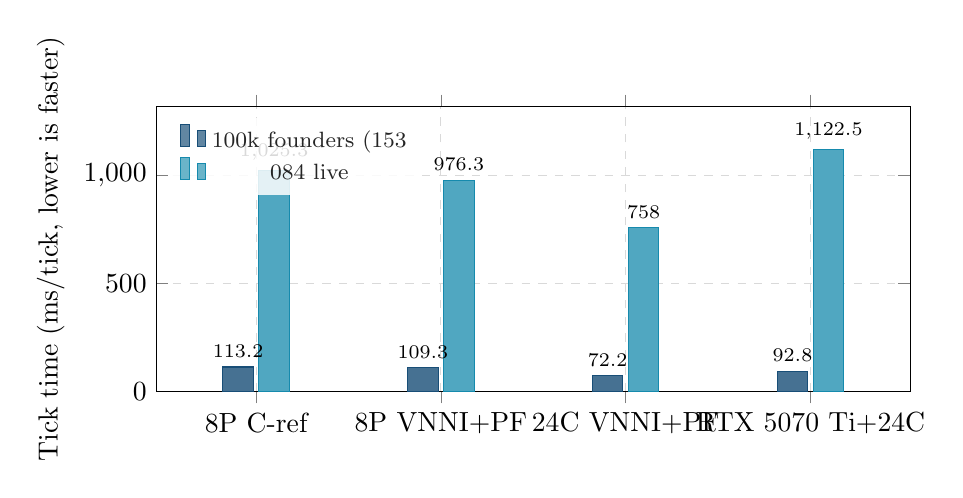
\begin{tikzpicture}
\begin{axis}[
  ybar,
  bar width=11pt,
  width=0.92\textwidth,
  height=5.2cm,
  ylabel={Tick time (ms/tick, lower is faster)},
  symbolic x coords={8P C-ref, 8P VNNI+PF, 24C VNNI+PF, RTX 5070 Ti+24C},
  xtick=data,
  ymin=0,
  ymax=1320,
  nodes near coords,
  nodes near coords style={font=\scriptsize, rotate=0, anchor=south},
  legend style={at={(0.02,0.96)}, anchor=north west, font=\footnotesize, draw=none, fill=white, fill opacity=0.85},
  enlarge x limits=0.18,
  grid=major,
  grid style={dashed, gray!30}
]
\addplot[fill=azblue!80, draw=azblue] coordinates {
  (8P C-ref, 113.2)
  (8P VNNI+PF, 109.3)
  (24C VNNI+PF, 72.2)
  (RTX 5070 Ti+24C, 92.8)
};
\addplot[fill=azteal!75, draw=azteal] coordinates {
  (8P C-ref, 1025.3)
  (8P VNNI+PF, 976.3)
  (24C VNNI+PF, 758.0)
  (RTX 5070 Ti+24C, 1122.5)
};
\legend{100k founders (153,084 live, hash \code{5b8110b324d2603f}), 1M founders (1,004,019 live, hash \code{31e5d00c106ce679})}
\end{axis}
\end{tikzpicture}
\caption{Measured bare-metal tick latency across substrates with bit-exact state-hash parity. At 1M founders, 24C AVX-VNNI+PF achieves 758.0 ms/tick (+35.3\% vs 8P C-ref), while PCIe staging and store compaction make RTX 5070 Ti offload slower (1,122.5 ms/tick) despite 0-fallback bit-exact execution.}
\label{fig:benchmarks}
\end{figure}

\subsection{Honest Disclosure of Negative Results and Tradeoffs}

Three negative or deferred outcomes are recorded explicitly in \code{docs\slsh TRIGGER-REGISTER.md} and \code{LIMITATIONS.md}:
\begin{enumerate}[leftmargin=1.8em,itemsep=2pt]
  \item \textbf{GPU PCIe/Compaction Bottleneck at 1M:} although the RTX~5070~Ti executes $4{,}999{,}522$ sparse brains across ticks with $0$ fallbacks and bit-exact hash \code{31e5d00c106ce679} (and HyperBrain 96-neuron parity \code{73a8d1f51b9556da}), synchronizing dirty variable-size creature store blocks across PCIe after two-half compaction yields $1{,}122.495$~ms/tick versus $757.988$~ms/tick on 24C AVX-VNNI CPU. Full GPU-resident world state remains open under \code{TR-05}.
  \item \textbf{Windows 2~MB Large Pages (\code{TR-03}):} \code{--large-pages} and \code{AZ\us WIN\us LARGE\us PAGES} are wired on \code{az\us run} and \code{az\us live}, but standard non-elevated Windows tokens lack \code{SeLockMemoryPrivilege}, so runs fall back cleanly to 4~KiB \code{VirtualLock} (\code{large\us pages=0}).
  \item \textbf{Unburned Confirmatory Seeds:} development lesion checks used seeds $1$--$24$ (where $23/23$ lesion bits altered state hashes and $8$ passed prespecified 64-tick primary thresholds); confirmatory reporting blocks $5001$--$5024$, $6001$--$6024$, and $6101$--$6124$ remain reserved pending long-horizon preregistered trials (\code{docs\slsh eval\slsh SEEDS.md}).
\end{enumerate}

\section{Unsolved Problems Mega-Atlas Non-Retirement Cross-Check}

Cross-mapping against the $1{,}900$-entry \code{unsolved-problems-mega-atlas} registry (\code{docs\slsh MEGA\us ATLAS\us CROSSCHECK.md}) establishes unequivocally that \textbf{$0 / 1{,}900$ overarching Mega-Atlas open problems are solved or retired} by \code{Asmodensius-Native}. Table~\ref{tab:atlas} records five related Atlas probes where this repository supplies a deterministic testbed or discrete invariant substrate while leaving every parent problem strictly \textbf{OPEN}.

\begin{table}[htbp]
\centering
\caption{Mega-Atlas Cross-Check Summary (0 / 1,900 Overarching Problems Retired).}
\label{tab:atlas}
\footnotesize
\setlength{\tabcolsep}{4pt}
\begin{tabularx}{\textwidth}{L{1.4cm}L{3.3cm}L{1.45cm}Y}
\toprule
\textbf{Atlas ID} & \textbf{Problem Title} & \textbf{Status} & \textbf{Scoped Role of Asmodensius-Native} \\
\midrule
\code{AI-045} & Open-Ended Artificial Life \& Unbounded Novelty & \textbf{OPEN} & Deterministic integer 3D ALife testbed (no fitness function) for future preregistered OEE trials~\cite{taylor2016open,packard2019overview}. \\
\code{BIO-001} & Abiogenesis: Origin of Life \& Genetic Code & \textbf{OPEN} & Discrete chemical-energy ledger (\code{NUT\us X}/\code{ORG\us Y}/\code{WST\us W}) and founder seeding; does not model prebiotic chemistry. \\
\code{BIO-008} & Major Evolutionary Transitions \& Complexity & \textbf{OPEN} & Colony commons, multicellular body parts, and lineage tracking; long-horizon transitions not yet demonstrated. \\
\code{SUB-047} & Hydrothermal Vents vs. Subaerial Warm Ponds & \textbf{OPEN} & Stylized seafloor vent mineral plumes (\code{az\us worldgen.c}); not a geochemical or laboratory discriminator. \\
\code{SYS-050} & Physical Intelligence \& Embodied Co-Design & \textbf{OPEN} & Coupled morphology, 64-channel sensing, and sparse recurrent brains under lesion tests; rigid-body compliance absent. \\
\bottomrule
\end{tabularx}
\end{table}

\section{Threats to Validity, Limitations, and Real-vs-Metaphor Boundary}

\begin{itemize}[leftmargin=1.8em,itemsep=2pt]
  \item \textbf{Real-vs-Metaphor Boundary (Law 8):} biological terminology in the codebase (``creature'', ``brain'', ``metabolism'', ``colony'', ``predation'') names deterministic integer data structures and state-transition rules. \code{Asmodensius-Native} makes \emph{zero} claims of consciousness, sentience, biological life, or AGI. The \code{butlin14} catalog~\cite{butlin2023consciousness} is strictly an engineering indicator scorecard, and \code{tk\us qsv}/\code{tk\us qgt} are purely classical fixed-point matrix routines with zero quantum physics or quantum speedup.
  \item \textbf{Formal-to-Binary Gap:} Lean~4.35.0 proves $30$ algebraic/protocol specifications over mathematical \code{Nat} and abstract types. It does not mechanically verify GCC/Clang C23 compilation (unlike a verified C compiler such as CompCert~\cite{leroy2009formal}), NASM instruction encodings, or NVIDIA PTX driver JIT translation; those layers are guarded empirically by $77/77$ CTest, UBSan traps, \code{core\us obj\us gate}, \code{avx\us stack\us gate}, and $164/164$ \code{test\us gpu}.
  \item \textbf{Single-Host Windows Scope:} the runtime targets Windows x86-64 on \code{Z:} (\code{VirtualLock}, \code{WaitOnAddress}, \code{BCryptGenRandom}) per project Law~10; Linux CI validates the 6-kernel Lean proof suite, Tectonic PDF, citation integrity, and repository standard audit while native engine execution requires Windows.
  \item \textbf{Open Trigger Register:} $12$ deferred items remain open in \code{docs\slsh TRIGGER-REGISTER.md}, including $>1\text{M}$ population scaling (\code{TR-02}), 2~MB large pages (\code{TR-03}), GPU-resident world state (\code{TR-05}), Intel NPU probes (\code{TR-06}), in-place store compaction (\code{TR-14}), and parallel birth commits (\code{TR-17}).
\end{itemize}

\section{Reproducibility, AI Disclosure, Authorship, and Licensing}

\subsection{Reproducibility}
From a clean clone, independent reviewers can verify every artifact via \code{justfile} or direct CLI commands documented in \code{REPLICATION.md}: (1) CMake + Ninja native build and \code{ctest --test-dir build/z --output-on-failure} on Windows; (2) 6-kernel Lean~4.35.0 replay under \code{lean/} (\code{lake build}, \code{lake build Challenge}, \code{VerifyAxioms.lean}, \code{lake check --paranoid}, and \code{lake comparator} with \code{comparator.json} in paranoid mode); (3) zero-overflow PDF and clean-room arXiv tarball build via \code{python -I scripts\slsh build\us paper.py}; and (4) live DOI and retraction verification via \code{python -I scripts\slsh check\us citations.py --live}. Cryptographic digests are recorded in \code{CHECKSUMS.sha256} and \code{data\slsh MANIFEST.sha256}.

\subsection{AI-Assistance Disclosure, CRediT, and Conflict of Interest}
\textbf{CRediT Authorship:} Alexander Stephen Donahue (Independent Researcher, Spokane, WA, USA; ORCID \code{0009-0006-8168-9648}) is the sole human author responsible for Conceptualization, Methodology, Software Architecture, Formal Verification Review, Validation, and Writing.

\textbf{AI-Assistance Disclosure:} AI coding assistants (Codex CLI, Claude Code, and Gemini-based agents) assisted with C23/NASM/PTX implementation iterations, Lean~4 tactic refactoring to Palomar module headers, LaTeX typesetting, and Build Standard scaffolding under human direction and Law-enforced audit gates. All reported claims are backed exclusively by deterministic machine execution ($77/77$ CTest, $164/164$ \code{test\us gpu}, $30/30$ Lean~4.35.0 multi-kernel checks, and live Crossref API verification). Full disclosure is maintained in \code{docs\slsh AI\us DISCLOSURE.md}.

\textbf{Conflict of Interest and Dual Licensing:} The author declares no competing financial interests and no external funding. No corporate entity holds rights to this work. Code, Lean proofs, and build scripts are licensed under \textbf{Apache-2.0} (\code{LICENSE}); this white paper, figures, documentation, and datasets are licensed under \textbf{CC-BY-4.0} (\code{LICENSE-DOCS}). Third-party MIT test-oracle provenance is documented in \code{THIRD\us PARTY\us NOTICES.md}.

\bibliographystyle{amsplain}
\bibliography{refs}

\end{document}
